\documentclass[12pt]{article}
\usepackage[left=2cm,right=2cm,top=2cm,bottom=2cm,bindingoffset=0cm]{geometry}
\usepackage[utf8x]{inputenc}
\usepackage[english,russian]{babel}
\usepackage{cmap}
\usepackage{amssymb}
\usepackage{amsmath}
\usepackage{url}
\usepackage{pifont}
\usepackage{tikz}
\usepackage{verbatim}

\usetikzlibrary{shapes,arrows}
\usetikzlibrary{positioning,automata}
\tikzset{every state/.style={minimum size=0.2cm},
initial text={}
}


\newenvironment{myauto}[1][3]
{
  \begin{center}
    \begin{tikzpicture}[> = stealth,node distance=#1cm, on grid, very thick]
}
{
    \end{tikzpicture}
  \end{center}
}


\begin{document}
\begin{center} {\LARGE Формальные языки} \end{center}

\begin{center} \Large домашнее задание до 23:59 16.03 \end{center}
\bigskip

\begin{enumerate}
  \item Доказать или опровергнуть свойство регулярных выражений:
  \[
    \forall p, q \text{ --- регулярные выражения}: (p \mid q)^* = p^*(qp^*)^*
  \]
  Доказательство.

  Выражение $(p \mid q)^*$ распознает любые строки, состоящие из p или q. 
  
  Рассмотрим $p^*(qp^*)^*$, выражение $(qp^*)^*$ распознает все строки, не начанающиеся с p, тогда $p*$ дополняет его. 
  Соответственно, правое выражение тоже распознает все строки, состоящие из p или q.

  \item Доказать или опровергнуть свойство регулярных выражений:
  \[
    \forall p, q \text{ --- регулярные выражения}: (p q)^* p = p (q p)^*
  \]

  Доказательство.
  
  Докажем с помощью построения минимального ДКА.

  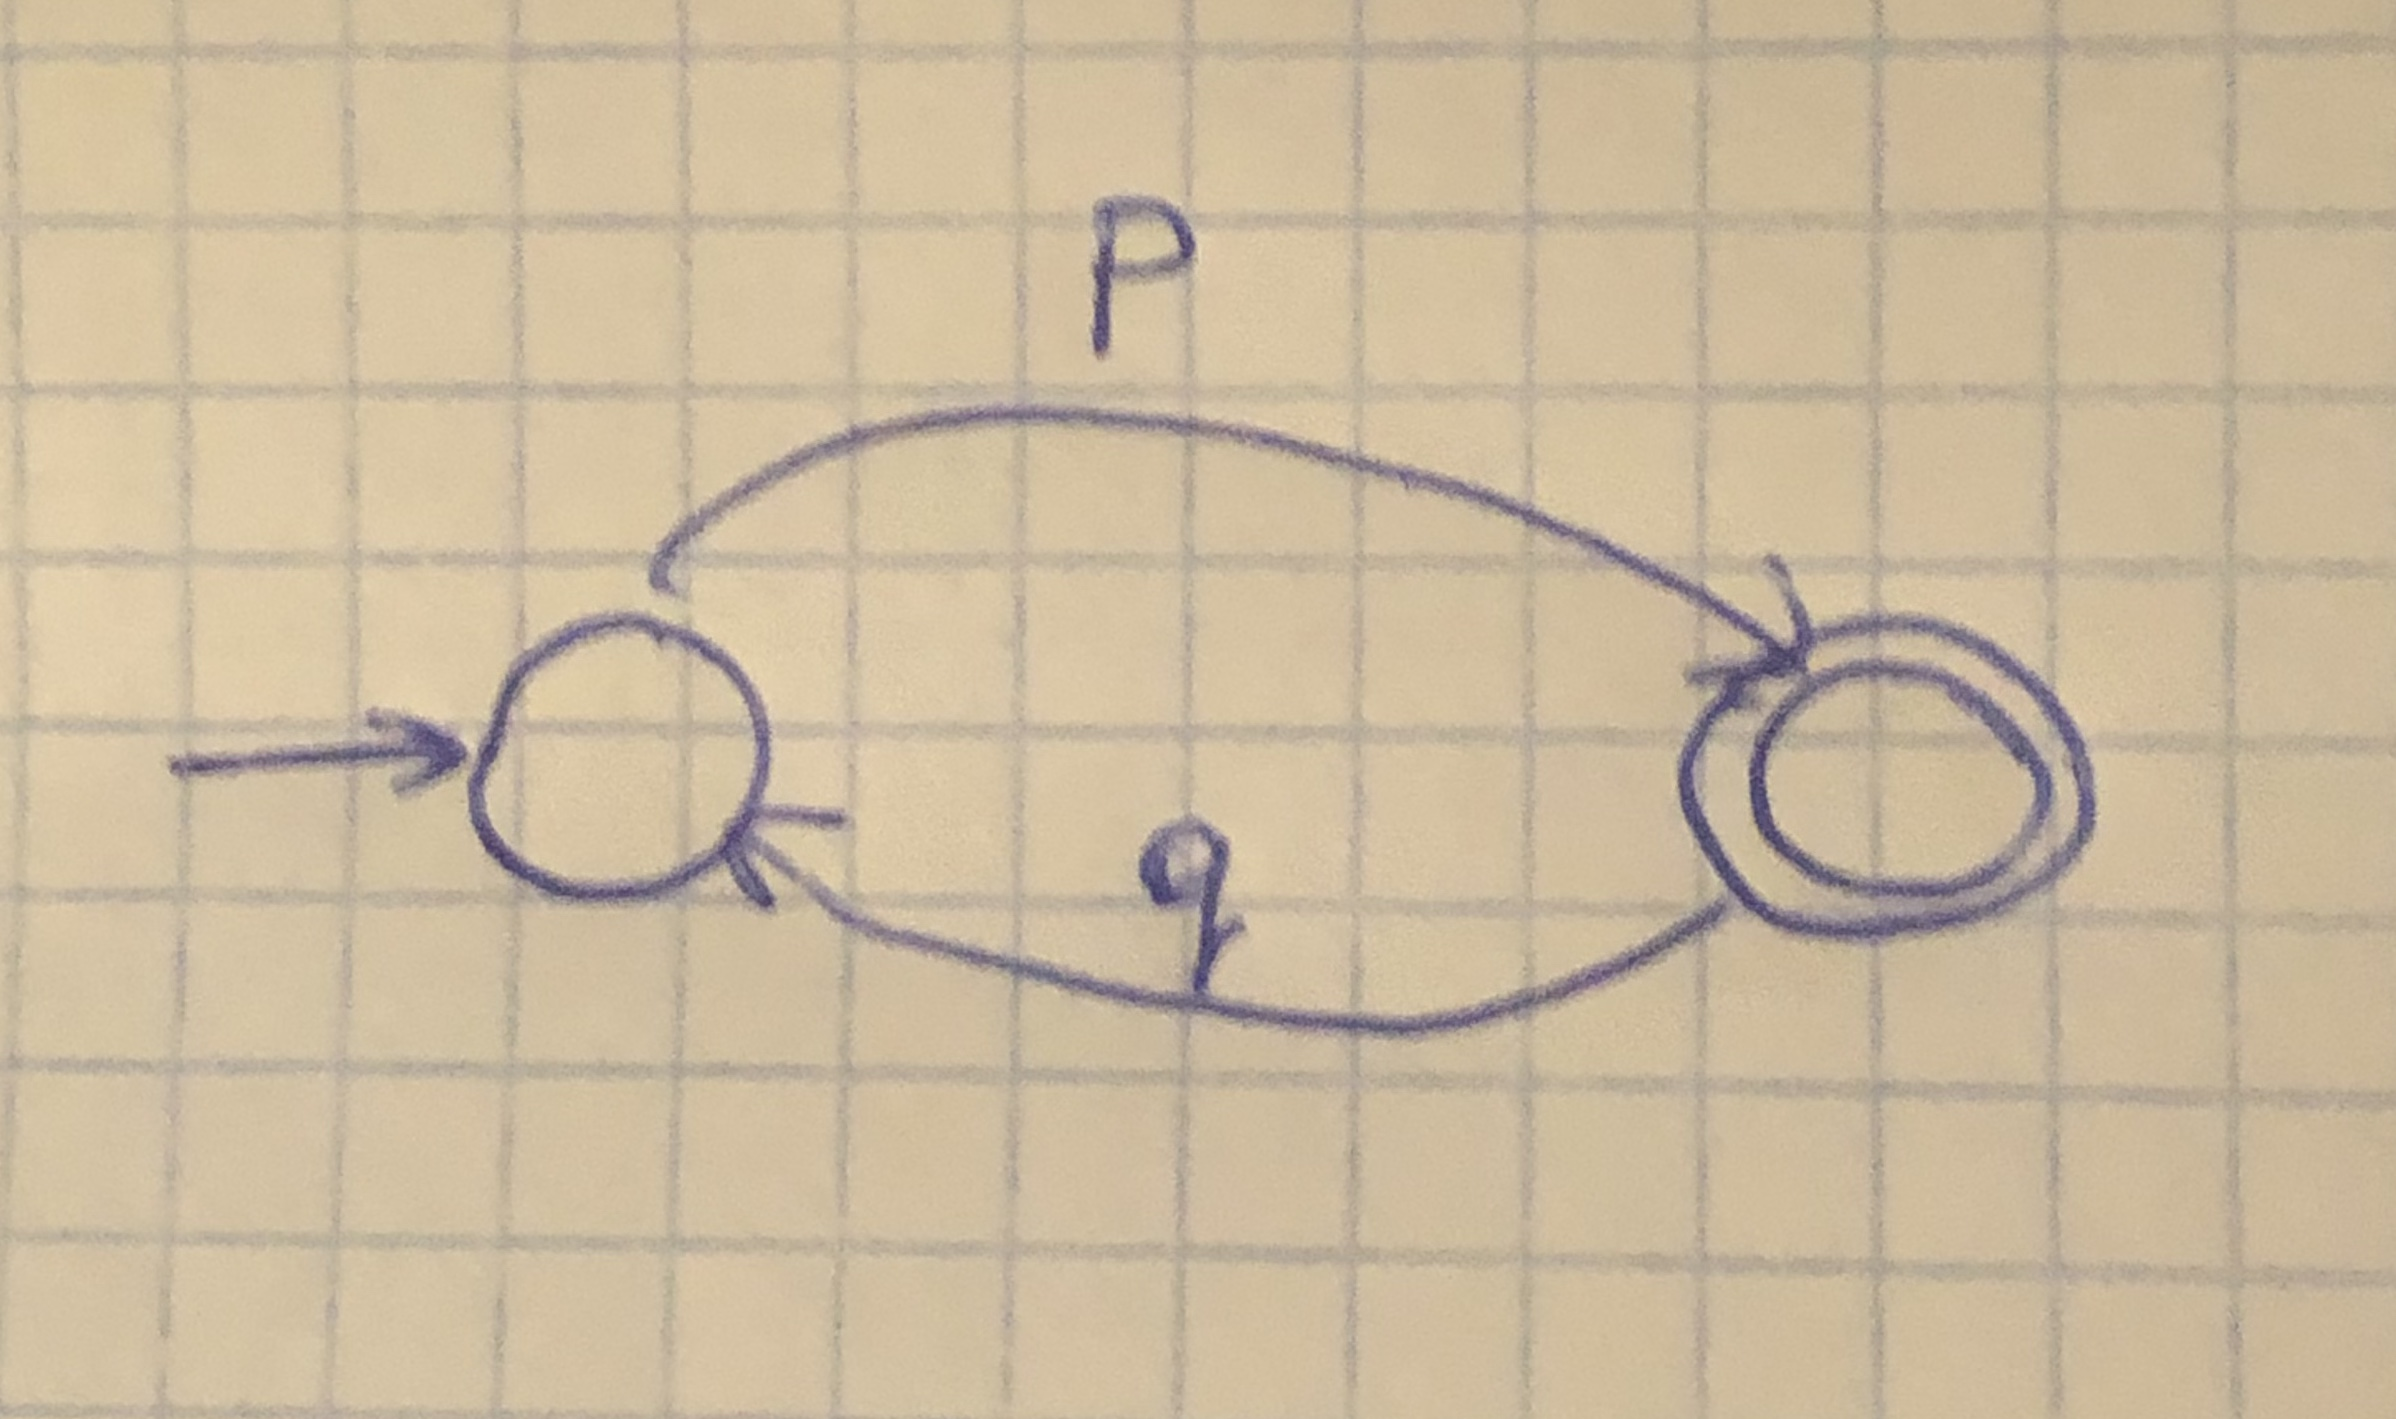
\includegraphics[width=0.5\linewidth]{IMG_7134.jpg}

  \item Доказать или опровергнуть свойство регулярных выражений:
  \[
    \forall p, q \text{ --- регулярные выражения}: (p q)^* = p^* q^*
  \]

  Неверно. Контрпример: правое вырашение принимает $p$, левое -- нет.

  \item Для регулярного выражения:
   \[ (a \mid b)^+ (aa \mid bb \mid abab \mid baba)^* (a \mid b)^+\]

  Построить эквивалентные:
  \begin{enumerate}
    \item Недетерминированный конечный автомат
    \item Недетерминированный конечный автомат без $\varepsilon$-переходов
    \item Минимальный полный детерминированный конечный автомат
  \end{enumerate}

\end{enumerate}

\end{document}
